\chapter{الأيونات والمحاليل الأيونية}\label{ch:g9:ions}

على مقعد في القاعة الرياضية مشروبان رائقان: قارورة مشروب رياضي يُباع
«لكهارله»، وكأس من الماء المحلّى بالسكر. وفي المختبر تُغمس في كل منهما
بالتناوب صفيحتان فلزيتان موصولتان ببطارية ومصباح صغير. في المشروب الرياضي
يضيء المصباح؛ وفي الماء المحلّى يبقى مطفأً. فثمة شيء في السائل الأول يحمل
شحنة كهربائية، والسكر لا يحملها. وهذا الشيء هو \omterm{def:g9:ions:ion}{الأيونات}.

\begin{recall}
في \omterm{def:g7:atoms-and-molecules:atom}{الذرة} \omterm{def:g9:inside-the-atom:nucleus}{نواة} فيها $Z$ بروتونًا، شحنة كل منها $+e$، وحولها $Z$
إلكترونًا، شحنة كل منها $-e$: \omterm{def:g7:atoms-and-molecules:atom}{فالذرة} متعادلة
(\cref{ch:g9:inside-the-atom}). \omterm{def:g6:solutions-and-solubility:solute}{والمذاب} الذائب في الماء يعطي \omterm{def:g6:solutions-and-solubility:solute}{محلولًا
مائيًا} (\cref{ch:g6:solutions-and-solubility}). \omterm{def:g7:identifying-substances:characteristic-test}{والاختبار المميِّز} يكشف
عن \omterm{def:g6:pure-substances-and-mixtures:species}{نوع كيميائي} بنتيجة مرئية
(\cref{ch:g7:identifying-substances}).
\end{recall}

\begin{omfigure}
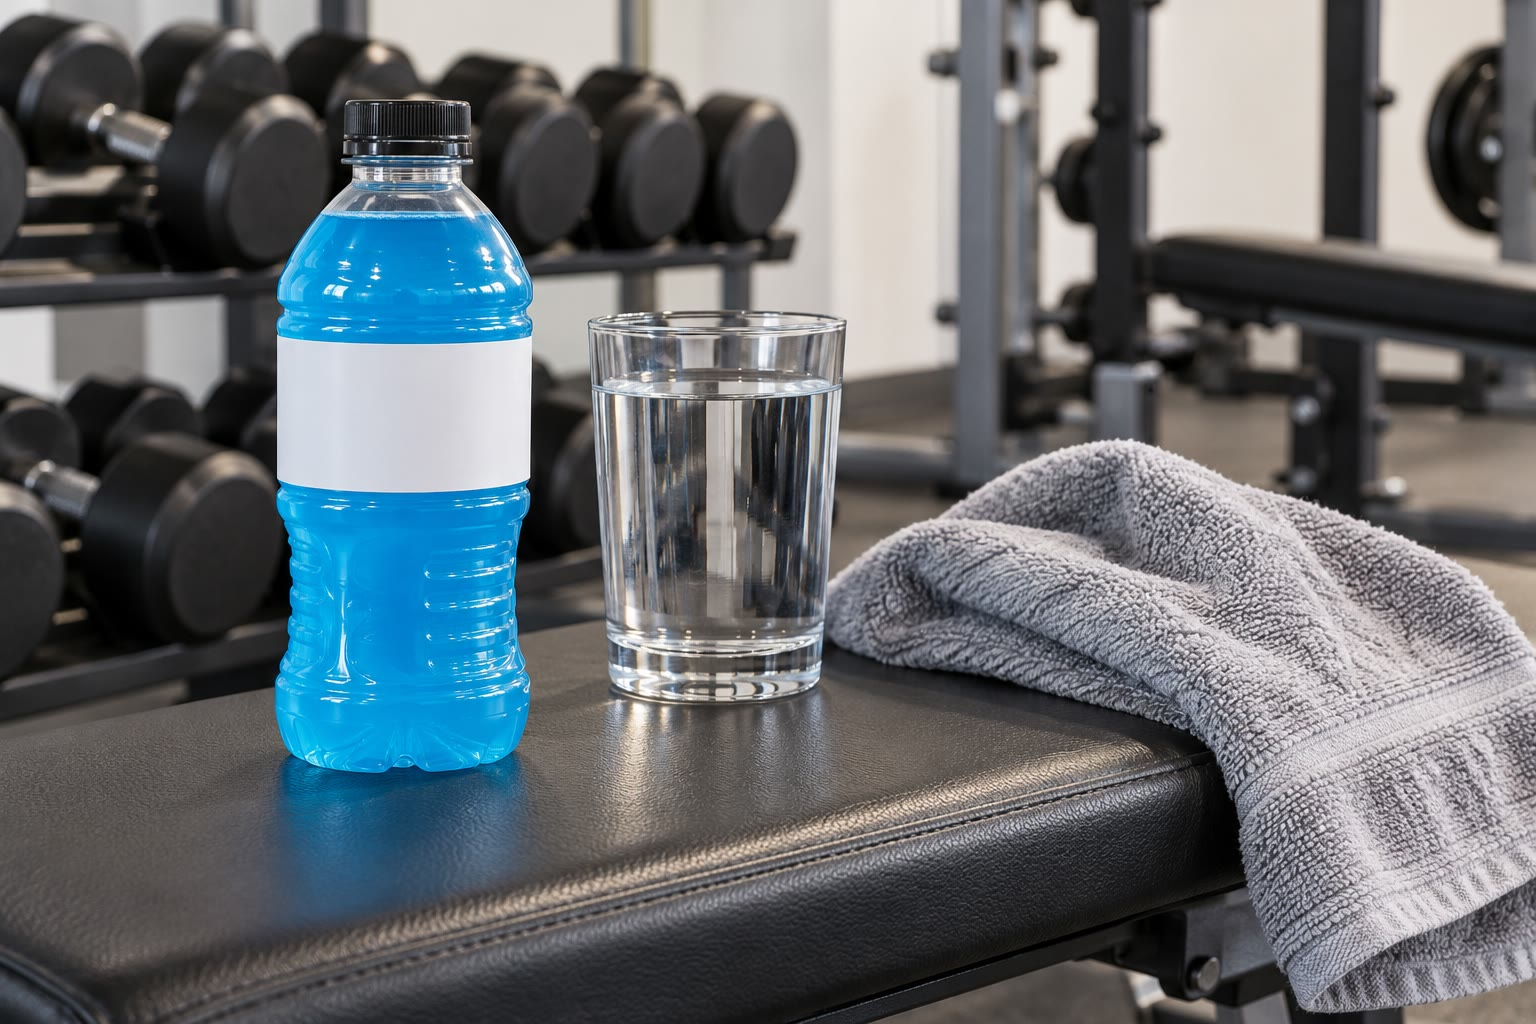
\includegraphics[width=0.5\linewidth]{images/book1/ai/g9-sports-drink.jpg}

{\small مشروب رياضي وكأس ماء: المشروب يحوي \omterm{def:g9:ions:ion}{أيونات}
ذائبة.}
\end{omfigure}

\section{ذرات تكتسب إلكترونات أو تفقدها}

\begin{definition}[الأيون والكاتيون والأنيون]\label{def:g9:ions:ion}
\emph{الأيون}\index{أيون} \omterm{def:g7:atoms-and-molecules:atom}{ذرة}، أو مجموعة من \omterm{def:g7:atoms-and-molecules:atom}{الذرات}، فقدت إلكترونًا أو أكثر
أو اكتسبته، فصارت تحمل شحنة كهربائية. والأيون ذو الشحنة الموجبة، الذي فقد
\omterm{def:g9:inside-the-atom:nucleus}{إلكترونات}، هو \emph{الكاتيون}\index{كاتيون}؛ والأيون ذو الشحنة السالبة،
الذي اكتسب \omterm{def:g9:inside-the-atom:nucleus}{إلكترونات}، هو \emph{الأنيون}\index{أنيون}. وتُكتب الشحنة في
أعلى يمين الصيغة: \ce{Na+}، \ce{Cu^{2+}}، \ce{Cl-}.
\end{definition}

\begin{example}[الصوديوم والكلور]\label{ex:g9:ions:na-cl}
\omterm{def:g7:atoms-and-molecules:atom}{ذرة} الصوديوم، وفيها 11 بروتونًا و11 إلكترونًا، تفقد إلكترونًا واحدًا: فتصير
\omterm{def:g9:ions:ion}{أيون} الصوديوم \ce{Na+}، وفيه 11 بروتونًا و10 \omterm{def:g9:inside-the-atom:nucleus}{إلكترونات}، وشحنته
$+1$:
\[
  \ce{Na -> Na+ + e-}.
\]
\omterm{def:g7:atoms-and-molecules:atom}{وذرة} الكلور، وفيها 17 بروتونًا و17 إلكترونًا، تكتسب إلكترونًا واحدًا: فتصير
\omterm{def:g9:ions:ion}{أيون} الكلوريد \ce{Cl-}، وفيه 17 بروتونًا و18 إلكترونًا:
\[
  \ce{Cl + e- -> Cl-}.
\]
\end{example}

\begin{omfigure}
\begin{tikzpicture}[font=\small]
  \foreach \x/\name/\p/\e/\ch/\col in {0/{ذرة الصوديوم}/11/11/0/omDef,
      3.7/{\foreignlanguage{arabic}{أيون الصوديوم \ce{Na+}}}/11/10/+1/omProp,
      8.0/{ذرة الكلور}/17/17/0/omDef, 11.7/{\foreignlanguage{arabic}{أيون الكلوريد \ce{Cl-}}}/17/18/$-1$/omProp} {
    \node[draw=\col, fill=\col!6, rounded corners=2pt, align=center, text width=2.4cm]
      at (\x,0) {\textbf{\name}\\ \foreignlanguage{arabic}{البروتونات: \babelsublr{\p}}\\ \foreignlanguage{arabic}{الإلكترونات: \babelsublr{\e}}\\ \foreignlanguage{arabic}{الشحنة: \babelsublr{\ch}}};
  }
  \draw[->, thick, omProp] (1.45,0) -- (2.25,0) node[midway, above, text=black,
    font=\footnotesize, align=center] {تفقد\\ 1 \ce{e-}};
  \draw[->, thick, omProp] (9.45,0) -- (10.25,0) node[midway, above, text=black,
    font=\footnotesize, align=center] {تكتسب\\ 1 \ce{e-}};
\end{tikzpicture}

{\small تصير \omterm{def:g7:atoms-and-molecules:atom}{ذرة} الصوديوم \omterm{def:g9:ions:ion}{أيون} صوديوم بفقدها إلكترونًا؛ وتصير \omterm{def:g7:atoms-and-molecules:atom}{ذرة} الكلور
\omterm{def:g9:ions:ion}{أيون} كلوريد باكتسابها إلكترونًا. ولا تتغير
\omterm{def:g9:inside-the-atom:proton}{البروتونات}.}
\end{omfigure}

\begin{proposition}[بعض الأيونات الشائعة]\label{prop:g9:ions:common}
\omterm{def:g9:ions:ion}{الأيونات} الأحادية \omterm{def:g7:atoms-and-molecules:atom}{الذرة} تتكوّن من \omterm{def:g7:atoms-and-molecules:atom}{ذرة} واحدة؛ \omterm{def:g9:ions:ion}{والأيونات} المتعددة \omterm{def:g7:atoms-and-molecules:atom}{الذرات} من
مجموعة من \omterm{def:g7:atoms-and-molecules:atom}{الذرات} تبقى متحدة:
\begin{center}
\small
\begin{tabular}{llll}
\hline
الكاتيونات & & الأنيونات & \\
\hline
الصوديوم & \ce{Na+} & الكلوريد & \ce{Cl-} \\
البوتاسيوم & \ce{K+} & الهيدروكسيد & \ce{OH-} \\
الكالسيوم & \ce{Ca^{2+}} & النترات & \ce{NO3-} \\
المغنيسيوم & \ce{Mg^{2+}} & الكربونات & \ce{CO3^{2-}} \\
النحاس (II) & \ce{Cu^{2+}} & الكبريتات & \ce{SO4^{2-}} \\
الحديد (II)، الحديد (III) & \ce{Fe^{2+}}، \ce{Fe^{3+}} & & \\
الزنك & \ce{Zn^{2+}} & & \\
الألومنيوم & \ce{Al^{3+}} & & \\
الأمونيوم & \ce{NH4+} & & \\
\hline
\end{tabular}
\end{center}
\end{proposition}

\section{المركبات الأيونية وصيغها}

\begin{definition}[المركب الأيوني]\label{def:g9:ions:ionic-compound}
\emph{المركب الأيوني}\index{مركب أيوني} مكوّن من كاتيونات وأنيونات بأعداد
تجعل المجموع غير مشحون. وتعطي صيغته نسبة \omterm{def:g9:ions:ion}{الأيونات}، دون شحناتها: \ce{NaCl}
لكلوريد الصوديوم، أي \ce{Na+} واحد لكل \ce{Cl-}؛ و\ce{CaCl2} لكلوريد
الكالسيوم، أي اثنان من \ce{Cl-} لكل \ce{Ca^{2+}}.
\end{definition}

\begin{method}[كتابة صيغة المركب الأيوني]\label{met:g9:ions:formula}
\begin{enumerate}
  \item اكتب الأيونين بشحنتيهما، \omterm{def:g9:ions:ion}{الكاتيون} أولًا.
  \item جد أصغر عدد من كل منهما يجعل الشحنة الكلية
        صفرًا.
  \item اكتب هذين العددين أدلةً سفلية؛ \omterm{def:g9:ions:ion}{والأيون} المتعدد \omterm{def:g7:atoms-and-molecules:atom}{الذرات} الذي يحتاج
        إلى \omterm{def:g7:atoms-and-molecules:formula}{دليل سفلي} يوضع بين قوسين.
\end{enumerate}
أكسيد الألومنيوم: \ce{Al^{3+}} و\ce{O^{2-}}؛ $2 \times (+3) + 3 \times
(-2) = 0$، إذن \ce{Al2O3}. هيدروكسيد الحديد (III): \ce{Fe^{3+}} وثلاثة
\ce{OH-}: \ce{Fe(OH)3}.
\end{method}

\begin{proposition}[الجسم الصلب الأيوني رصّ من الأيونات]\label{prop:g9:ions:solid}
في بلورة الملح تتناوب \omterm{def:g9:ions:ion}{أيونات} الصوديوم \omterm{def:g9:ions:ion}{وأيونات} الكلوريد في رصّ منتظم ثلاثي
الأبعاد، وكل \omterm{def:g9:ions:ion}{أيون} محاط \omterm{def:g9:ions:ion}{بأيونات} ذات شحنة معاكسة تثبته في مكانه. وحبة ملح
الطعام الواحدة تحوي مليارات المليارات منها؛ وشكلها المكعب يعكس الرصّ
المكعب.
\end{proposition}

\begin{omfigure}
\begin{minipage}[b]{0.5\linewidth}\centering
\begin{tikzpicture}[font=\small]
  \foreach \i in {0,...,5} \foreach \j in {0,...,4} {
    \pgfmathtruncatemacro\pp{mod(\i+\j,2)}
    \ifnum\pp=0 \node[aNa, minimum size=5mm] at (0.62*\i,0.62*\j) {};
    \else \node[aCl, minimum size=7.4mm] at (0.62*\i,0.62*\j) {};\fi
  }
\end{tikzpicture}

{\small طبقة واحدة من بلورة ملح: \omterm{def:g9:ions:ion}{أيونات} الصوديوم (بنفسجية، أصغر) \omterm{def:g9:ions:ion}{وأيونات}
الكلوريد (خضراء) تتناوب.}
\end{minipage}\hfill
\begin{minipage}[b]{0.3\linewidth}\centering
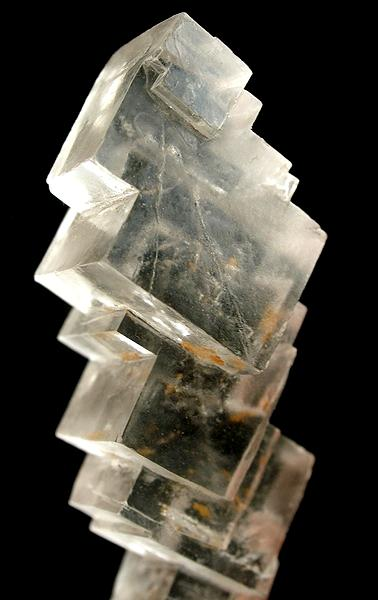
\includegraphics[height=4.6cm]{images/book1/halite.jpg}

{\small الهاليت، ملح الصخر الطبيعي. تصوير: روبرت م.~لافينسكي،
CC BY-SA 3.0.}
\end{minipage}
\end{omfigure}

\section{المحاليل الأيونية توصل الكهرباء}

\begin{notation}[رمز الحالة (aq)]\label{not:g9:ions:aq}
يُميَّز \omterm{def:g9:ions:ion}{الأيون} أو \omterm{def:g7:atoms-and-molecules:molecule}{الجزيء} الذائب في الماء بالرمز (aq)، أي مائي:
\ce{Na+(aq)}، \ce{Cl-(aq)}.
\end{notation}

\begin{proposition}[المحاليل الأيونية توصل الكهرباء]\label{prop:g9:ions:conduct}
حين \omterm{def:g2:mixing-and-dissolving:dissolve}{يذوب} \omterm{def:g9:ions:ionic-compound}{مركب أيوني} في الماء تنفصل أيوناته وتتحرك بحرية في \omterm{def:g2:mixing-and-dissolving:dissolve}{المحلول}: فالماء
المالح يحوي \ce{Na+(aq)} و\ce{Cl-(aq)}. \omterm{def:g9:ions:ion}{والأيونات} المتحركة تحمل الشحنة
الكهربائية، ولذلك يوصل \omterm{def:g2:mixing-and-dissolving:dissolve}{المحلول} الأيوني الكهرباء. أما \omterm{def:g2:mixing-and-dissolving:dissolve}{محلول} السكر، الذي لا
تحمل جزيئاته شحنة، فلا يوصلها؛ ولا يوصلها الماء البالغ النقاء.
\end{proposition}

\begin{inthelab}[أي السوائل يوصل الكهرباء؟]
يصل المعلم في دارة صفيحتين فلزيتين وبطارية منخفضة التوتر ومصباحًا صغيرًا؛
ثم تُغمس الصفيحتان بالتناوب في الماء المقطر، والماء المحلّى، والماء المالح،
\omterm{def:g2:mixing-and-dissolving:dissolve}{ومحلول} كبريتات النحاس، وتُشطفان بين كل غمسة وأخرى. ولا يضيء المصباح إلا مع
المحلولين الأيونيين.
\end{inthelab}

\begin{omfigure}
\begin{tikzpicture}[font=\small, scale=1.1]
  \foreach \xs/\lit/\lab in {0/1/{ماء مالح: يضيء المصباح}, 5.2/0/{ماء محلّى: يبقى مطفأً}} {
    \begin{scope}[xshift=\xs cm]
      \pic[transform shape] at (2,0) {beaker={0.7}{omWater!80}};
      \fill[black!45] (1.6,0.25) rectangle (1.7,2.6);
      \fill[black!45] (2.3,0.25) rectangle (2.4,2.6);
      \ifnum\lit=1 \fill[yellow!70, opacity=0.8] (3.4,3.0) circle (0.42);\fi
      \draw (1.65,2.6) -- (1.65,3.6) to[battery1] (3.4,3.6) -- (3.4,3.4)
        to[lamp] (3.4,2.6) -- (2.35,2.6);
      \node[anchor=north, align=center] at (2,-0.15) {\lab};
    \end{scope}
  }
\end{tikzpicture}

{\small اختبار التوصيل: مع الماء المالح تحمل \omterm{def:g9:ions:ion}{الأيونات} التيار فيضيء المصباح؛
والماء المحلّى لا يحوي \omterm{def:g9:ions:ion}{أيونات} فيبقى المصباح
مطفأً.}
\end{omfigure}

\section{اختبارات الترسيب للتعرف على الأيونات}

\begin{definition}[الراسب]\label{def:g9:ions:precipitate}
حين يُخلط محلولان، قد يكوّن \omterm{def:g9:ions:ion}{كاتيون} من أحدهما \omterm{def:g9:ions:ion}{وأنيون} من الآخر مركبًا أيونيًا
لا \omterm{def:g2:mixing-and-dissolving:dissolve}{يذوب}. فيظهر جسمًا صلبًا دقيقًا يعكّر السائل ثم يترسب: وهو
\emph{الراسب}\index{راسب}. ويسمى التفاعل
\emph{تفاعل ترسيب}\index{تفاعل ترسيب}.
\end{definition}

\begin{proposition}[اختبارات الأيونات الشائعة]\label{prop:g9:ions:tests}
بضع قطرات من \omterm{def:g2:mixing-and-dissolving:dissolve}{محلول} \omterm{def:g7:identifying-substances:characteristic-test}{كاشف} تكفي للتعرف على \omterm{def:g9:ions:ion}{أيون} بلون \omterm{def:g9:ions:precipitate}{الراسب} الذي
يكوّنه:
\begin{center}
\small
\begin{tabular}{llll}
\hline
\omterm{def:g9:ions:ion}{الأيون} المبحوث عنه & \omterm{def:g7:identifying-substances:characteristic-test}{الكاشف} & \omterm{def:g9:ions:precipitate}{الراسب} & اللون \\
\hline
النحاس (II) \ce{Cu^{2+}} & هيدروكسيد الصوديوم & \ce{Cu(OH)2} & أزرق \\
الحديد (II) \ce{Fe^{2+}} & هيدروكسيد الصوديوم & \ce{Fe(OH)2} & أخضر \\
الحديد (III) \ce{Fe^{3+}} & هيدروكسيد الصوديوم & \ce{Fe(OH)3} & برتقالي بني \\
الزنك \ce{Zn^{2+}} & هيدروكسيد الصوديوم & \ce{Zn(OH)2} & أبيض \\
الألومنيوم \ce{Al^{3+}} & هيدروكسيد الصوديوم & \ce{Al(OH)3} & أبيض \\
الكلوريد \ce{Cl-} & نترات الفضة & \ce{AgCl} & أبيض، يسودّ في الضوء \\
\hline
\end{tabular}
\end{center}
\end{proposition}

\begin{example}[كتابة تفاعل ترسيب]\label{ex:g9:ions:equation}
لا تُكتب إلا \omterm{def:g9:ions:ion}{الأيونات} التي تكوّن الجسم الصلب؛ أما \omterm{def:g9:ions:ion}{الأيونات} الأخرى فتبقى ذائبة
ولا تشارك في التفاعل:
\[
  \ce{Cu^{2+}(aq) + 2OH-(aq) -> Cu(OH)2(s)}, \qquad
  \ce{Ag+(aq) + Cl-(aq) -> AgCl(s)}.
\]
\end{example}

\begin{omfigure}
\begin{tikzpicture}[font=\small, scale=0.95]
  \foreach \k/\pc/\lab in {0/blue!60/{\foreignlanguage{arabic}{\ce{Cu^{2+}}: أزرق}}, 1/green!45!black!70/{\foreignlanguage{arabic}{\ce{Fe^{2+}}: أخضر}},
      2/orange!70!brown/{\foreignlanguage{arabic}{\ce{Fe^{3+}}: برتقالي}\\بني}, 3/white!85!black/{\foreignlanguage{arabic}{\ce{Zn^{2+}}: أبيض}},
      4/white!85!black/{\foreignlanguage{arabic}{\ce{Al^{3+}}: أبيض}}, 5/white!80!black/{\foreignlanguage{arabic}{\ce{Cl-}: أبيض}}} {
    \pic[transform shape] at (\k*2.3,0) {testtube={0.5}{omWater!60}};
    \pic[transform shape] at (\k*2.3,0) {testtube={0.14}{\pc}};
    \node[anchor=north, align=center, font=\footnotesize, text width=2cm] at (\k*2.3,-0.15) {\lab};
  }
\end{tikzpicture}

{\small رواسب تتكوّن مع هيدروكسيد الصوديوم (الأنابيب الخمسة الأولى) ومع
نترات الفضة (الأنبوب الأخير).}
\end{omfigure}

\begin{safety}{\ghs[0.82cm]{GHS05}\ghs[0.82cm]{GHS07}}
% ledger: ghs:NaOH, ghs:AgNO3
هيدروكسيد الصوديوم: يسبب حروقًا جلدية شديدة وتلفًا للعينين، وقد يكون أكّالًا
للفلزات (GHS05)؛ ويهيّج الجلد والعينين وهو مخفف (GHS07). ونترات الفضة،
\omterm{def:g7:identifying-substances:characteristic-test}{كاشف} الكلوريد، مؤكسد وأكّال وشديد السمية للأحياء المائية. نظارات واقية
وقفازات؛ ويصرف المعلم الكواشف قطرة قطرة.
\end{safety}

\begin{method}[اختبار أيون]\label{met:g9:ions:test}
\begin{enumerate}
  \item صب قليلًا من \omterm{def:g2:mixing-and-dissolving:dissolve}{المحلول} المراد اختباره في أنبوب اختبار.
  \item أضف \omterm{def:g7:identifying-substances:characteristic-test}{الكاشف} قطرة قطرة.
  \item سجّل لون \omterm{def:g9:ions:precipitate}{الراسب} إن ظهر وقارنه بالجدول.
  \item استنتج، وتذكّر أن الاختبار يتعرف على \omterm{def:g9:ions:ion}{أيون} لا على مركب: \omterm{def:g2:mixing-and-dissolving:dissolve}{فمحلول}
        كلوريد الحديد (III) يعطي اختبار \ce{Fe^{3+}} واختبار \ce{Cl-}
        كليهما.
\end{enumerate}
\end{method}

\section{تمارين}

\begin{exercise}[$\star$]\label{exo:g9:ions:1}
ما \omterm{def:g9:ions:ion}{الأيون}؟ وما الفرق بين \omterm{def:g9:ions:ion}{الكاتيون} \omterm{def:g9:ions:ion}{والأنيون}؟
\end{exercise}

\begin{exercise}[$\star$]\label{exo:g9:ions:2}
\omterm{def:g7:atoms-and-molecules:atom}{ذرة} مغنيسيوم (12 بروتونًا) تفقد إلكترونين. اكتب صيغة \omterm{def:g9:ions:ion}{الأيون} المتكوّن، وأعطِ
عدد بروتوناته وإلكتروناته.
\end{exercise}

\begin{exercise}[$\star$]\label{exo:g9:ions:3}
اكتب صيغ كلوريد البوتاسيوم وكلوريد المغنيسيوم وأكسيد الكالسيوم (\omterm{def:g9:ions:ion}{أيون}
الأكسيد: \ce{O^{2-}}).
\end{exercise}

\begin{exercise}[$\star$]\label{exo:g9:ions:4}
لماذا يوصل الماء المالح الكهرباء بينما لا يوصلها الماء المحلّى؟
\end{exercise}

\begin{exercise}[$\star\star$]\label{exo:g9:ions:5}
اكتب صيغ كبريتات النحاس (II) وكلوريد الألومنيوم وكربونات
الصوديوم.
\end{exercise}

\begin{exercise}[$\star\star$]\label{exo:g9:ions:6}
يعطي هيدروكسيد الصوديوم المضاف إلى \omterm{def:g2:mixing-and-dissolving:dissolve}{محلول} راسبًا برتقاليًا بنيًا. أي \omterm{def:g9:ions:ion}{أيون}
يحوي \omterm{def:g2:mixing-and-dissolving:dissolve}{المحلول}؟ اكتب معادلة \omterm{def:g9:ions:precipitate}{تفاعل
الترسيب}.
\end{exercise}

\begin{exercise}[$\star\star$]\label{exo:g9:ions:7}
كم إلكترونًا يحمل \omterm{def:g9:ions:ion}{أيون} الكبريتات \ce{SO4^{2-}} زيادة على عدد
بروتوناته؟ \omterm{def:g9:ions:ion}{وأيون} النترات \ce{NO3-}؟
\end{exercise}

\begin{exercise}[$\star\star$]\label{exo:g9:ions:8}
يعطي \omterm{def:g2:mixing-and-dissolving:dissolve}{محلول} راسبًا أبيض مع نترات الفضة وراسبًا أزرق مع هيدروكسيد الصوديوم.
سمِّ \omterm{def:g9:ions:ionic-compound}{المركب الأيوني} الذائب واكتب
صيغته.
\end{exercise}

\begin{exercise}[$\star\star$]\label{exo:g9:ions:9}
انظر إلى شكل طبقة بلورة الملح. كم جارًا ذا شحنة معاكسة \omterm{def:g9:ions:ion}{لأيون} في وسط الطبقة
داخل هذه
الطبقة؟
\end{exercise}

\begin{exercise}[$\star\star$]\label{exo:g9:ions:10}
اكتب معادلة ترسيب هيدروكسيد الحديد (II) من \omterm{def:g9:ions:ion}{أيونات}
\ce{Fe^{2+}} و\ce{OH-}.
\end{exercise}

\begin{exercise}[$\star\star\star$]\label{exo:g9:ions:11}
مسحوق أبيض قد يكون كلوريد الزنك أو كلوريد الصوديوم. إذا أُذيب في الماء
أعطى راسبًا أبيض مع هيدروكسيد الصوديوم. فأيهما هو؟
اكتب المعادلة.
\end{exercise}

\begin{exercise}[$\star\star\star$]\label{exo:g9:ions:12}
في بلورة كلوريد الكالسيوم، كم \omterm{def:g9:ions:ion}{أيون} كلوريد يوجد لكل 1000 \omterm{def:g9:ions:ion}{أيون} كالسيوم؟
تحقق من أن البلورة متعادلة.
\end{exercise}

\section{مسألة: البئر الصدئة}

\begin{problem}[{مسألة نهاية الأسبوع --- بقع برتقالية في مغسلة بيت ريفي،
واختباران، وعدد أيونات الحديد في لتر من ماء البئر}]
\label{pb:g9:ions:1}
يترك ماء بئر بيت ريفي بقعًا برتقالية في المغسلة. فيتلقى مختبر عيّنة منه.
والماء المسحوب حديثًا رائق؛ ومع هيدروكسيد الصوديوم يعطي راسبًا أخضر، يصير
برتقاليًا بنيًا في أقل من ساعة عند السطح، حيث يلامس \omterm{def:g4:air-a-mixture-of-gases:air}{الهواء}. ويقيس المختبر
\qty{0.30}{mg} من الحديد، على شكل \omterm{def:g9:ions:ion}{أيونات} حديد، في اللتر. خذ كتلة
\omterm{def:g9:inside-the-atom:proton}{النوكليون} \qty{1.67e-27}{kg}، و56 نوكليونًا \omterm{def:g7:atoms-and-molecules:atom}{لذرة}
الحديد.

\medskip
\noindent\textbf{الجزء الأول --- الاختبارات.}
\begin{enumerate}
  \item أي \omterm{def:g9:ions:ion}{أيون} يبيّنه \omterm{def:g9:ions:precipitate}{الراسب} الأخضر؟ أعطِ صيغة
        \omterm{def:g9:ions:precipitate}{الراسب}.
  \item أي \omterm{def:g9:ions:ion}{أيون} يبيّنه \omterm{def:g9:ions:precipitate}{الراسب} البرتقالي البني؟ أعطِ
        صيغته.
  \item يختلف \omterm{def:g9:ions:ion}{أيون} الحديد (II) \omterm{def:g9:ions:ion}{وأيون} الحديد (III) \omterm{def:g9:inside-the-atom:nucleus}{بإلكترون} واحد.
        أيهما فيه \omterm{def:g9:inside-the-atom:nucleus}{إلكترونات} أكثر؟ وكم إلكترونًا في كل منهما
        (الحديد: $Z = 26$)؟
  \item اكتب معادلة ترسيب هيدروكسيد الحديد (III).
\end{enumerate}

\medskip
\noindent\textbf{الجزء الثاني --- البقع.}
\begin{enumerate}[resume]
  \item في المغسلة يتعكّر الماء الرائق ببطء ويصير برتقاليًا. أي \omterm{def:g9:ions:ion}{أيون} يحمل
        الماء حين يخرج من البئر، وأي \omterm{def:g9:ions:ion}{أيون} ينتهي إلى
        حمله؟
  \item اكتب صيغة \omterm{def:g9:ions:ionic-compound}{المركب الأيوني} الذي تكوّنه \omterm{def:g9:ions:ion}{أيونات} الحديد (III)
        \omterm{def:g9:ions:ion}{وأيونات} الهيدروكسيد، وتحقق من أنه متعادل.
  \item هل يمكن إزالة حديد الماء \omterm{def:g3:separating-mixtures:filter}{بترشيح} الماء لحظة خروجه من البئر؟
        وبعد أن يصير برتقاليًا؟ علّل.
  \item هل الماء الذي يحوي \omterm{def:g9:ions:ion}{أيونات} الحديد \omterm{def:g6:pure-substances-and-mixtures:pure-substance}{مادة نقية}؟ وهل هو \omterm{def:g6:pure-substances-and-mixtures:homogeneous}{خليط
        متجانس}؟
\end{enumerate}

\medskip
\noindent\textbf{الجزء الثالث --- عدّ \omterm{def:g9:ions:ion}{الأيونات}.}
\begin{enumerate}[resume]
  \item احسب كتلة \omterm{def:g7:atoms-and-molecules:atom}{ذرة} الحديد بالكيلوغرام.
  \item حوّل \qty{0.30}{mg} إلى الكيلوغرام.
  \item لماذا يجوز أن نعدّ كتلة \omterm{def:g9:ions:ion}{أيون} الحديد مساوية لكتلة \omterm{def:g7:atoms-and-molecules:atom}{ذرة}
        الحديد؟
  \item احسب عدد \omterm{def:g9:ions:ion}{أيونات} الحديد في لتر من ماء البئر.
\end{enumerate}
\end{problem}
